\chapter{Divide and Conquer}

    \section{Recursive Algorithms}
    Before discussing divide-and-conquer algorithms, it is essential to understand the concept of recursive algorithms. A recursive algorithm is one that calls itself one or more times to solve a problem. The core idea is to divide the problem into smaller and simpler sub-problems, solve them individually, and then combine the solutions.
    
    A classical example is calculating the power of a number. For instance, calculating \(2^3\) can be done recursively by breaking it down as:
    \[
    2^3 = 2 \times 2^2 = 2 \times (2 \times 2^1)
    \]
    
    Recursion differs from iteration. While iteration involves loops, recursion involves a function calling itself. Iteration is generally more efficient in terms of constant factors, but recursion can simplify the design of an algorithm.
    
    \subsection{Base Case in Recursion}
    
    It is crucial that every recursive algorithm includes a base case, which provides a condition to stop the recursion. Without a base case, the algorithm would continue to call itself infinitely, leading to a stack overflow.
    
    \subsection{Execution Stack}
    Each time a recursive call is made, the current state of the function is saved in the execution stack (a LIFO structure). This is similar to a stack of objects where new items are added to the top. Once a function completes, its state is removed from the stack, and the previous function call is resumed. 
    
    For example, the execution stack for the function \texttt{RECURSIVE-POWER(2,3)} works as follows:
    
    \begin{itemize}
        \item The initial call \texttt{RECURSIVE-POWER(2,3)} leads to the call \texttt{RECURSIVE-POWER(2,2)}.
        \item Then, \texttt{RECURSIVE-POWER(2,2)} calls \texttt{RECURSIVE-POWER(2,1)}.
        \item Once \texttt{RECURSIVE-POWER(2,1)} returns the result, the previous calls are resumed until the final result is computed.
    \end{itemize}
    
    \section{Divide-and-Conquer Strategy}
    
    The divide-and-conquer strategy is commonly used in recursive algorithms. This strategy involves three main steps:
    \begin{itemize}
        \item \textbf{Divide:} Break the problem into smaller sub-problems.
        \item \textbf{Conquer:} Solve each sub-problem recursively.
        \item \textbf{Combine:} Combine the solutions of the sub-problems to form the final solution.
    \end{itemize}
    
    A classical example of this strategy is the \textbf{Merge-Sort} algorithm.
    
    \subsection{Merge-Sort Algorithm}
    
    Merge-sort is a sorting algorithm that follows the divide-and-conquer paradigm. Here are the steps:
    \begin{enumerate}
        \item Assume we have an unordered sequence of \(n\) elements.
        \item \textbf{Divide:} Split the sequence into two halves, each of length \(n/2\).
        \item \textbf{Conquer:} Sort both halves recursively using merge-sort.
        \item \textbf{Combine:} Merge the two sorted halves into one sorted sequence.
    \end{enumerate}
    
    The key part of the algorithm is the \textbf{combine} step, where two sorted arrays are merged.
    \begin{figure}[h!]
        \centering
        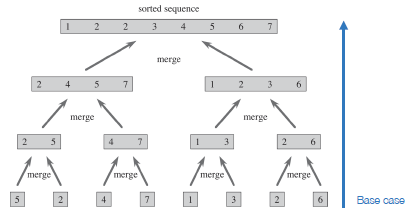
\includegraphics[width=0.75\linewidth]{immagini/merge_sort.png}
    \end{figure}
    \subsubsection{Merge-Sort Pseudo code}
    
    \begin{verbatim}
    MERGE-SORT(A, p, r)
        if p >= r
            return
        q = (p + r) / 2
        MERGE-SORT(A, p, q)
        MERGE-SORT(A, q+1, r)
        MERGE(A, p, q, r)
    \end{verbatim}
    
    Here, \(p\) and \(r\) represent the indices of the first and last elements of the array, and \(q\) is the middle index. The array is recursively split and sorted, and finally, the \texttt{MERGE} procedure combines the results.
    
    \subsubsection{Merge Procedure Pseudo code}
    
    \begin{verbatim}
    MERGE(A, p, q, r)
        n1 = q - p + 1
        n2 = r - q
        let L[1..n1+1] and R[1..n2+1] be new arrays
        for i = 1 to n1
            L[i] = A[p + i - 1]
        for j = 1 to n2
            R[j] = A[q + j]
        L[n1+1] = +infinite
        R[n2+1] = +infinite
        i = 1
        j = 1
        for k = p to r
            if L[i] <= R[j]
                A[k] = L[i]
                i = i + 1
            else
                A[k] = R[j]
                j = j + 1
    \end{verbatim}
    
    The \texttt{MERGE} function combines two sorted sub-arrays, \(L\) and \(R\), into a single sorted array. The use of sentinel values (\(\infty\)) ensures that the merging process can terminate correctly without additional checks.
    
    \section{Cost Analysis of Merge-Sort}
    The cost of Merge-Sort can be analyzed using recurrence relations. Here's the step-by-step breakdown:
    
    \subsection{Step 1: Divide the Array}
    
    Each time we divide the array, the size of the problem is halved. This results in two sub-problems of size \(n/2\). The time required to divide the array into two halves is constant, specifically \(\Theta(1)\), since it only involves calculating the midpoint \(q = (p + r) / 2\).
    
    \subsection{Step 2: Conquer the sub-problems}
    
    The two sub-problems are solved recursively, and the time to solve each sub-problem is given by the same merge-sort process. Therefore, the time required for solving both halves is \(T(n/2)\).
    
    \subsection{Step 3: Combine the Results (Merge Step)}
    
    The \texttt{MERGE} function takes \(\Theta(n)\) time because it processes all elements of the two sub-arrays, comparing and merging them into a single array. The merging process requires one pass through the elements, resulting in linear time complexity.
    
    \subsection{Overall Recurrence Relation}
    
    The time complexity of merge-sort can be described by the following recurrence relation:
    \[
    T(n) = 2T\left(\frac{n}{2}\right) + \Theta(n)
    \]
    This relation reflects the fact that we are solving two sub-problems of size \(n/2\), and the merging step takes \(\Theta(n)\) time.
    
    \subsection{Solving the Recurrence Relation}
    
    To solve this recurrence relation, we can use the \textbf{recursion tree method} or the \textbf{master theorem}. Let's go through the steps:
    \begin{enumerate}
        \item Recursive Expansion: Start by expanding the recurrence relation:
       \[
       T(n) = 2T\left(\frac{n}{2}\right) + \Theta(n)
       \]
       \[
       = 2\left(2T\left(\frac{n}{4}\right) + \Theta\left(\frac{n}{2}\right)\right) + \Theta(n)
       \]
       \[
       = 4T\left(\frac{n}{4}\right) + 2\Theta\left(\frac{n}{2}\right) + \Theta(n)
       \]
       \[
       = 8T\left(\frac{n}{8}\right) + 4\Theta\left(\frac{n}{4}\right) + 2\Theta\left(\frac{n}{2}\right) + \Theta(n)
       \]
       After expanding \(k\) times, we obtain:
       \[
       T(n) = 2^k T\left(\frac{n}{2^k}\right) + \sum_{i=0}^{k-1} 2^i \Theta\left(\frac{n}{2^i}\right)
       \] 
        \item Base Case:
       The base case occurs when the size of the sub-problem becomes 1, i.e., when \(n/2^k = 1\), which implies \(k = \log_2 n\). Substituting this into the expansion:
       \[
       T(n) = 2^{\log_2 n} T(1) + \sum_{i=0}^{\log_2 n - 1} 2^i \Theta\left(\frac{n}{2^i}\right)
       \]
       Since \(T(1)\) is a constant, we get:
       \[
       T(n) = n \cdot \Theta(1) + \sum_{i=0}^{\log_2 n - 1} \Theta(n)
       \]
        \item Sum Simplification:
       The sum simplifies to:
       \[
       \sum_{i=0}^{\log_2 n - 1} \Theta(n) = \log_2 n \cdot \Theta(n)
       \]
        \item Final Time Complexity:
       Therefore, the total time complexity is:
       \[
       T(n) = \Theta(n) + \log_2 n \cdot \Theta(n) = \Theta(n \log n)
       \]
    \end{enumerate}
        
    \subsection{Summary of Merge-Sort Complexity}
    
    Merge-Sort has a time complexity of \(\Theta(n \log n)\), which is optimal for comparison-based sorting algorithms. This time complexity holds for both the average and worst cases due to the divide-and-conquer structure, where the number of levels in the recursion tree is \(\log_2 n\), and each level performs \(\Theta(n)\) work for merging. The height of the tree is $h = log_2 n + 1$ and it has $n$ leaves.

\section{Recursion Tree Method for Complexity Analysis}

The recursion tree method is a visual tool to help analyze the complexity of recursive functions. Let’s consider the following exercises to explore this method in detail.

\subsection{Exercise 1: Analyzing \( T(n) = 3T\left(\frac{n}{4}\right) + \Theta(n^2) \)}
Given the recurrence relation:
\[
T(n) = 3T\left(\frac{n}{4}\right) + c n^2
\]
where \(c > 0\), \(a = 3\) is the number of subproblems, and \(b = 4\) represents the factor by which the problem size is reduced. The initial cost function \(cn^2\) is quadratic, meaning that the cost at each level will follow this quadratic pattern as the problem size decreases.

\subsection{Step-by-Step Analysis Using Recursion Tree}
\begin{enumerate}
    \item \textbf{Root Level}: At the root, the cost is \(cn^2\).

    \item \textbf{First Level of Subproblems}: We divide the problem into three subproblems, each of size \(n/4\), with cost:
   \[
   3 \cdot \left(\frac{n}{4}\right)^2 \cdot c = \frac{3}{16} n^2 c
   \]

    \item \textbf{Second Level}: Each subproblem of size \(n/4\) is divided again, resulting in three more subproblems per branch. The cost at this level becomes:
   \[
   \left(\frac{3}{16}\right)^2 n^2 c
   \]

    \item \textbf{Recursive Pattern}: We continue this process until reaching the leaves of the recursion tree, where the cost is constant (\(T(1)\)).
\end{enumerate}


\subsection{Calculating Total Cost}

The height of the tree is:
\[
h = \log_b n = \log_4 n
\]
and the number of leaves at the final level is approximately \(n\).

The total cost \(T(n)\) is the sum of the costs across each level:
\[
T(n) = \sum_{i=0}^{\log_4 n - 1} \left(\frac{3}{16}\right)^i \cdot c \, n^2 + \Theta(n^{\log_4 3})
\]

We can approximate this sum with an infinite geometric series:
\[
T(n) < \sum_{i=0}^{\infty} \left(\frac{3}{16}\right)^i \cdot c \, n^2
\]

Using the formula for the sum of an infinite geometric series \(\sum_{k=0}^{\infty} x^k = \frac{1}{1-x}\) for \(|x| < 1\), we get:
\[
T(n) < \frac{1}{1 - \frac{3}{16}} \cdot c \, n^2 + \Theta(n^{\log_4 3}) = \frac{16}{13} c \, n^2 + \Theta(n^{\log_4 3})
\]
Thus, we conclude:
\[
T(n) = O(n^2)
\]

\begin{center}
    \textbf{Recursion Tree for \(T(n) = 3T\left(\frac{n}{4}\right) + \Theta(n^2)\)}
\end{center}

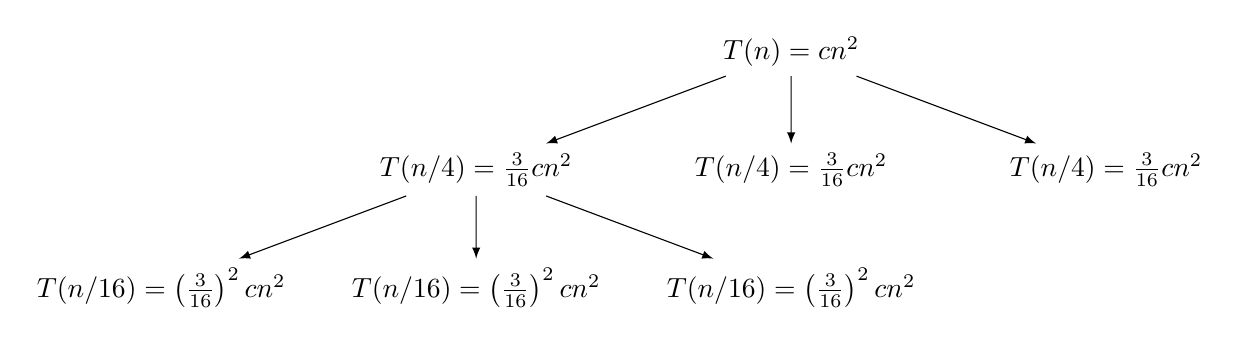
\begin{tikzpicture}
    [level distance=1.5cm, sibling distance=4cm, edge from parent/.style={draw,-latex}]
    \node { \( T(n) = cn^2 \) }
        child { node { \( T(n/4) = \frac{3}{16} cn^2 \) }
            child { node { \( T(n/16) = \left(\frac{3}{16}\right)^2 cn^2 \) } }
            child { node { \( T(n/16) = \left(\frac{3}{16}\right)^2 cn^2 \) } }
            child { node { \( T(n/16) = \left(\frac{3}{16}\right)^2 cn^2 \) } }
        }
        child { node { \( T(n/4) = \frac{3}{16} cn^2 \) } }
        child { node { \( T(n/4) = \frac{3}{16} cn^2 \) } };
\end{tikzpicture}

\subsection{Exercise 2: Analyzing \( T(n) = T\left(\frac{n}{3}\right) + T\left(\frac{2n}{3}\right) + cn \)}

Given the recurrence relation:
\[
T(n) = T\left(\frac{n}{3}\right) + T\left(\frac{2n}{3}\right) + cn
\]
\begin{enumerate}
    \item Root Level: At the root, the cost is \(cn\).
    \item Division into Subproblems: We divide the problem into subproblems of size \(n/3\) and \(2n/3\), each with cost proportional to \(cn\). 
    \item Continuing the Division: This is an unbalanced tree, as the \(2n/3\) branch will continue dividing for more levels than the \(n/3\) branch.
\end{enumerate}

Since the right branch (\(2n/3\)) divides more slowly, it will dominate the total cost. Therefore, we approximate the cost by following the longer branch.

\subsection{Calculating Height and Total Cost}

The height \(h\) of the tree based on the \(2n/3\) branch is:
\[
h = \log_{3/2} n
\]
Since each level has a cost \(cn\), the total cost is:
\[
T(n) = cn \cdot \log_{3/2} n = O(n \log n)
\]

\begin{center}
    \textbf{Partial Recursion Tree for \(T(n) = T\left(\frac{n}{3}\right) + T\left(\frac{2n}{3}\right) + cn\)}


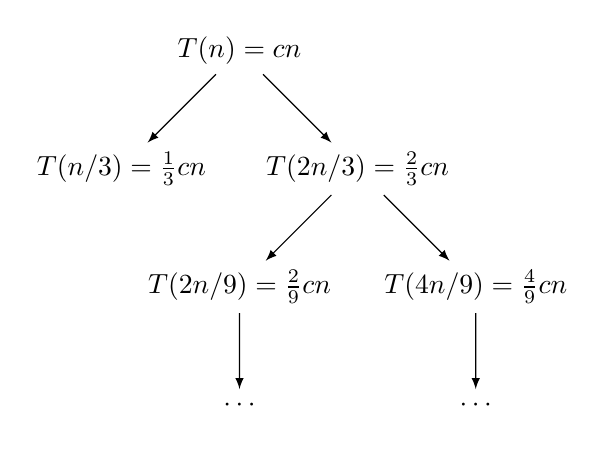
\begin{tikzpicture}
    [level distance=1.5cm, sibling distance=3cm, edge from parent/.style={draw,-latex}]
    \node { \( T(n) = cn \) }
        child { node { \( T(n/3) = \frac{1}{3} cn \) } }
        child { node { \( T(2n/3) = \frac{2}{3} cn \) }
            child { node { \( T(2n/9) = \frac{2}{9} cn \) }
                child { node { \(\cdots\) } }
            }
            child { node { \( T(4n/9) = \frac{4}{9} cn \) }
                child { node { \(\cdots\) } }
            }
        };
\end{tikzpicture}
\end{center}
\subsection{Summary}

In general, for a recurrence relation \( T(n) = a T\left(\frac{n}{b}\right) + \Theta(n^\alpha) \):
\begin{itemize}
    \item The recursion tree height is \( h = \log_b n \).
    \item The cost at each level is determined by the number of subproblems \(a\), the size reduction factor \(b\), and the initial complexity \(\alpha\).
    \item The total cost is derived from the sum of work at each level, up to the leaves.
\end{itemize}

\section{Exercise: Algorithm with Complexity \(\Theta(n \log n)\)}

Given a set \(S\) of \(n\) integers and another integer \(X\), determine if there exists a pair of elements in \(S\) whose sum equals \(X\). Note that we only need to find one such pair if it exists; it does not matter which pair.

A straightforward brute-force approach would involve two nested loops: for each element \(y \in S\), check if there exists another element \(w \in S\) such that \(y + w = X\). However, this approach has a time complexity of \(\Theta(n^2)\), which is suboptimal.

\subsection{Optimized Approach}
We aim to achieve a time complexity of \(\Theta(n \log n)\). Since sorting algorithms like merge-sort have this complexity, we can leverage sorting in our solution.

If there exist elements \(y, w \in S\) such that \(y + w = X\), then:
\[
w = X - y
\]
Define a new set \(S'\) as follows:
\[
            S' = \{z = X - y \mid y \in S\}
            \]
\begin{itemize}
    \item Sort \(S\) and \(S'\) using merge-sort, each with a time complexity of \(\Theta(n \log n)\).
    \item Merge \(S\) and \(S'\) into a new sequence \(S''\).
    \item Check if there exists an element in \(S\) that appears in \(S''\).
\end{itemize}

\subsection{Complexity Analysis}
\begin{itemize}
    \item Creating \(S'\) has a linear cost: \(\Theta(n)\).
    \item Sorting \(S\) and \(S'\) requires \(\Theta(n \log n)\).
    \item Merging \(S\) and \(S'\) takes linear time: \(\Theta(n)\).
    \item Checking for duplicate elements in \(S''\) also has a linear cost: \(\Theta(n)\).
\end{itemize}

Therefore, the total time complexity is:
\[
\Theta(n) + 2 \Theta(n \log n) = \Theta(n \log n)
\]

\section{Exercise: Finding an Element in a Sequence}

Given a sequence \(S\) of integers and an integer \(X\), determine whether \(X \in S\) and return the index \(i\) such that \(S[i] = X\).

\subsection{Linear Search}
If \(S\) is unordered, we must scan the entire sequence, resulting in a time complexity of \(\Theta(n)\). This is known as the linear scan.

\subsection{Binary Search}
If \(S\) is ordered, we can use binary search, which divides the search interval in half each step:
\begin{enumerate}
    \item Define two indices, \( \text{low} \) and \( \text{high} \).
    \item  Compute the midpoint as:
   \[
   \text{mid} = \left\lfloor \frac{\text{high} + \text{low}}{2} \right\rfloor
   \]
    \item If \(X < S[\text{mid}]\), continue searching in the left half \([ \text{low}, \text{mid} - 1 ]\).
    \item If \(X > S[\text{mid}]\), search in the right half \([ \text{mid} + 1, \text{high} ]\).
    \item If \(X = S[\text{mid}]\), return \(\text{mid}\).
\end{enumerate}
Each division reduces the search space by half, leading to a logarithmic time complexity: \(\Theta(\log n)\), which matches the height of a binary tree.

\subsection{Iterative Binary Search Algorithm}

\begin{verbatim}
def iterative_binary_search(S, X, low, high):
    while low <= high:
        mid = (high + low) // 2  # Equivalent to the floor of (high + low) / 2
        if S[mid] == X:
            return mid
        elif S[mid] < X:
            low = mid + 1
        else:
            high = mid - 1
    return None  # Return None if X is not found
\end{verbatim}

The \texttt{None} return indicates that the element was not found.

\subsection{Complexity Analysis}
The recurrence relation for the binary search is:
\[
T(n) = T\left(\frac{n}{2}\right) + \Theta(1)
\]
since each iteration reduces the problem size by half with a constant operation. Solving this recurrence, we find:
\[
T(n) = \Theta(\log n)
\]

\newpage
